\documentclass[tikz]{standalone}
\usepackage{amsmath}
\definecolor{bgdark}{HTML}{171D2B}
\definecolor{aksen}{HTML}{F7B538}
\definecolor{biru}{HTML}{4FA3E3}
\definecolor{merah}{HTML}{E36B4F}
\definecolor{hijau}{HTML}{59C77F}
\definecolor{abu}{HTML}{9AA3B5}
\begin{document}
\pagecolor{bgdark}
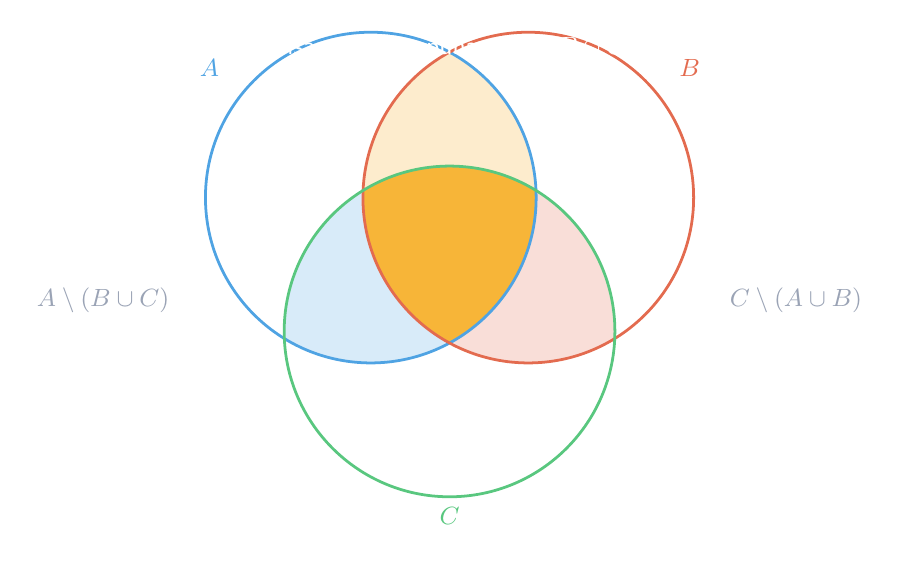
\begin{tikzpicture}[text=white, font=\sffamily\small, line width=1pt]
  \def\r{2.1}
  \coordinate (A) at (-1.0, 0.7);
  \coordinate (B) at ( 1.0, 0.7);
  \coordinate (C) at ( 0.0,-1.0);
  \begin{scope}
    \clip (A) circle (\r);
    \fill[aksen!25] (B) circle (\r);
    \fill[biru!22]  (C) circle (\r);
  \end{scope}
  \begin{scope}
    \clip (B) circle (\r);
    \fill[merah!22] (C) circle (\r);
  \end{scope}
  \begin{scope}
    \clip (A) circle (\r);
    \clip (B) circle (\r);
    \fill[aksen!55] (C) circle (\r);
  \end{scope}
  \begin{scope}
    \clip (A) circle (\r);
    \clip (B) circle (\r);
    \clip (C) circle (\r);
    \fill[aksen] (current bounding box.south west) rectangle (current bounding box.north east);
  \end{scope}
  \draw[biru]  (A) circle (\r);
  \draw[merah] (B) circle (\r);
  \draw[hijau] (C) circle (\r);
  \node[biru]  at (-3.05, 2.35) {$A$};
  \node[merah] at ( 3.05, 2.35) {$B$};
  \node[hijau] at ( 0.0,-3.35) {$C$};
  \node[abu] at (-4.4,-0.6) {$A\setminus(B\cup C)$};
  \node[abu] at ( 4.4,-0.6) {$C\setminus(A\cup B)$};
  \node[white] at ( 0.0, 2.6) {irisan tiga himpunan: $A\cap B\cap C$};
\end{tikzpicture}
\end{document}
